\documentclass[12pt,a4paper]{article}
\usepackage{ctex}
\usepackage{graphicx}
\usepackage{geometry}
\usepackage{array}
\usepackage{setspace}
\usepackage{xeCJK}
\usepackage{indentfirst}
\usepackage{amsmath}
\usepackage{float}
\usepackage{subfigure}
\usepackage{booktabs}
\usepackage{multirow}
\usepackage{caption}

% 设置页边距
\geometry{left=2.5cm,right=2.5cm,top=2.5cm,bottom=2.5cm}

% 设置行距
\linespread{1.0}

% 取消首行缩进
\setlength{\parindent}{0em}

% 设置默认字体为宋体小四
\setCJKmainfont[BoldFont=SimHei]{SimSun}
\zihao{-4}

\begin{document}

% 页眉部分
\begin{center}
  \begin{tabular}{p{0.3\textwidth}p{0.7\textwidth}}
    
\includegraphics[width=0.3\textwidth]{assets/scut_logo.png} &
    \zihao{3}\songti\textbf{大学物理实验（一）实验报告}
  \end{tabular}
\end{center}

% 标题
\begin{center}
  {\zihao{-3}\songti\textbf{马吕斯定律验证}}
\end{center}

\vspace{0.8cm}

% 学生信息表格（改为下划线样式）
\noindent \begin{tabular}{@{}llll}
24级\underline{\makebox[3cm][c]{x}} 班 & 
姓名\underline{\makebox[3cm][c]{Pinco Li}} & 
小组序号\underline{\makebox[3cm][c]{x}} \\[2ex]
\end{tabular}

\noindent \begin{tabular}{@{}llll}
实验日期 2025 年\underline{\makebox[1cm][c]{3}} 月 \underline{\makebox[1cm][c]{21}} 日 
& 第 4 周 
& 星期\underline{\makebox[2cm][c]{五}} 
& 指导老师\underline{\makebox[2cm][c]{x}} \\[2ex]
\end{tabular}

\noindent 同组同学\underline{\makebox[5cm][c]{x}}

\vspace{0.8cm}

% 实验目的部分标题
\textbf{一、实验目的}

a. 学习使用偏振光实验装置。

b. 深入理解光的偏振性质。

c. 测量验证马吕斯定律。

\vspace{0.5cm}
\textbf{二、实验仪器}

\textbf{1. OEX-PSP偏振光测试仪}

完整套装包括半导体激光器、导轨、带转盘的起偏器、光强检测器和调节装置。如图1所示
\begin{figure}[H]
    \begin{minipage}[t]{0.5\linewidth}
        \centering
        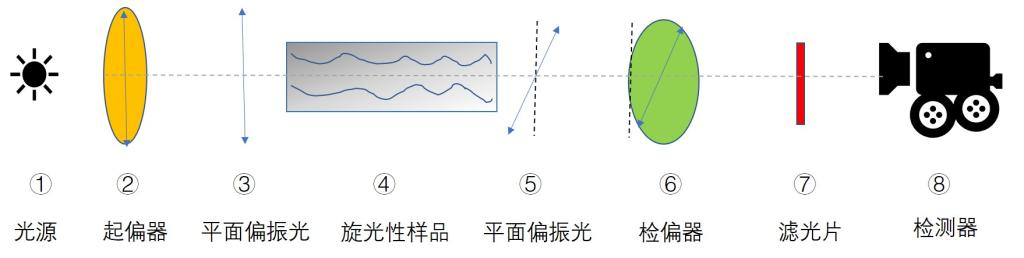
\includegraphics[clip,scale=0.1]{assets/fig1.jpg}
        \caption{OEX-PSP偏振光测试仪}
        \label{figure.1}
    \end{minipage}
    \begin{minipage}[t]{0.5\linewidth}
        \centering
        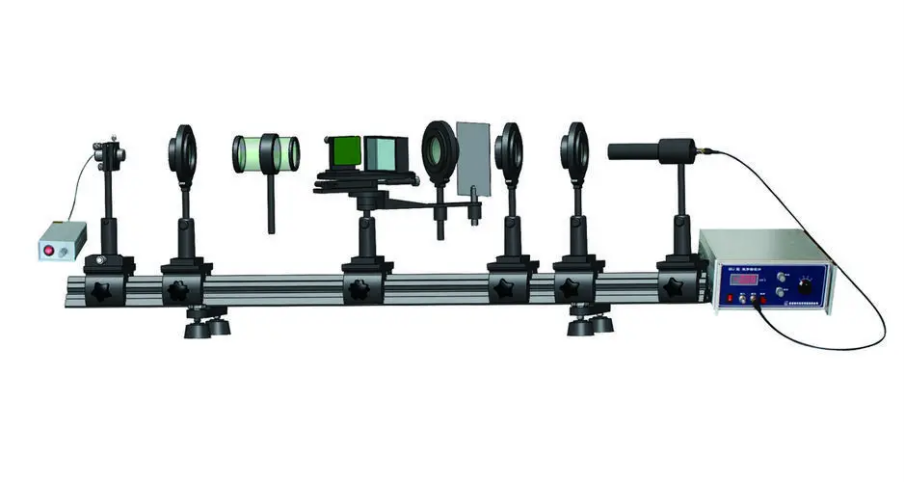
\includegraphics[clip,scale=0.8,trim={0 30 0 0}]{assets/fig2.png}
        \caption{物理演示图}
        \label{figure.2}
    \end{minipage}
\end{figure}

\textbf{2. 偏振器和检偏器}

用于产生和检测偏振光的装置，可以旋转以改变偏振方向。

\begin{figure}[H]
    \centering
    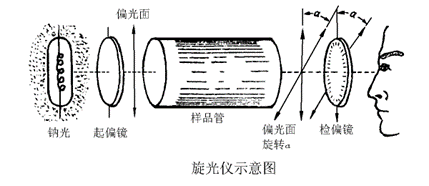
\includegraphics[clip,scale=1,trim={0 22 0 0}]{assets/fig3.png}
    \caption{实验仪器各部分详细说明}
    \label{figure.3}
\end{figure}

\vspace{0.5cm}
\textbf{三、实验原理}

\textbf{1. 光的偏振性}

光是电磁波，由于电磁波对物质的作用主要是电场，光学中将电场强度E称为光矢量。在垂直于光波传播方向的平面内，光矢量可能有不同的振动方向，光矢量保持在某一确定振动方向的状态通常称为偏振状态。如果光在传播过程中，光矢量保持固定平面振动，这种振动状态称为平面振动状态，该平面称为振动面（见图4）。此时光矢量在垂直于传播方向的平面内的投影是一条直线，因此也称为线偏振状态。如果光矢量围绕传播方向旋转，其端点描绘出一个圆的轨迹，这种偏振状态称为圆偏振状态。如果光矢量的端点沿椭圆旋转，则变成椭圆偏振状态。（见图5）
\begin{figure}[H]
    \begin{minipage}[t]{0.5\linewidth}
        \centering
        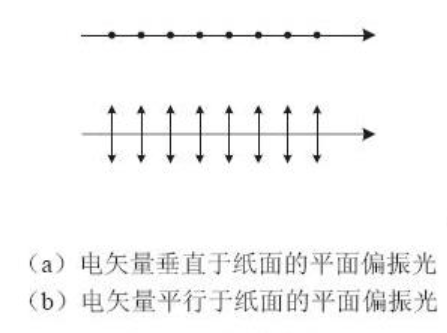
\includegraphics[clip,scale=1,trim={0 60 0 0}]{assets/fig4.png}
        \caption{平面偏振光}
        \label{figure.4}
    \end{minipage}
    \begin{minipage}[t]{0.5\linewidth}
        \centering
        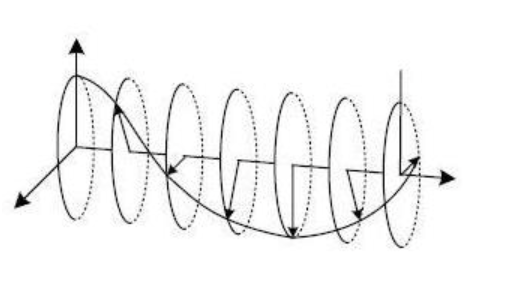
\includegraphics[clip,scale=0.8]{assets/fig5.png}
        \caption{椭圆偏振光}
        \label{figure.5}
    \end{minipage}
\end{figure}

\textbf{2. 偏振器}

虽然普通光源发出的是自然光，但自然界中存在各种偏振光。广泛使用的偏振光装置是人工偏振器，它利用二色性获得偏振光（某些各向同性介质，在某种作用下，会表现出各向异性，能强烈吸收入射光矢量在某一方向的分量并传递其垂直分量，从而将入射自然光变为偏振光，具有这种性质的介质称为二色性）。偏振装置可用于将自然光变为平面偏振光——偏振，或识别线偏振光、自然光和部分偏振光——偏振检测。用于偏振的偏振器称为起偏器，用于偏振检测的偏振装置称为检偏器。实际上，起偏器和检偏器是通用的。

\textbf{3. 马吕斯定律}

\textbf{(1) 关于马吕斯定律}

马吕斯定律指出，通过分析器的平面偏振光的强度随着偏振器平面与分析器透射轴之间角度的余弦平方而变化。

\begin{figure}[H]
\begin{minipage}[t]{0.5\linewidth}
    \centering
    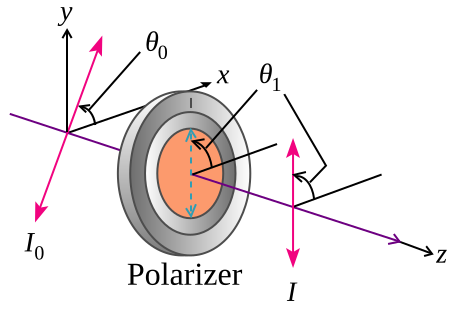
\includegraphics[clip,scale=0.31]{assets/fig6.png}
\end{minipage}
\begin{minipage}[t]{0.5\linewidth}
    \centering
    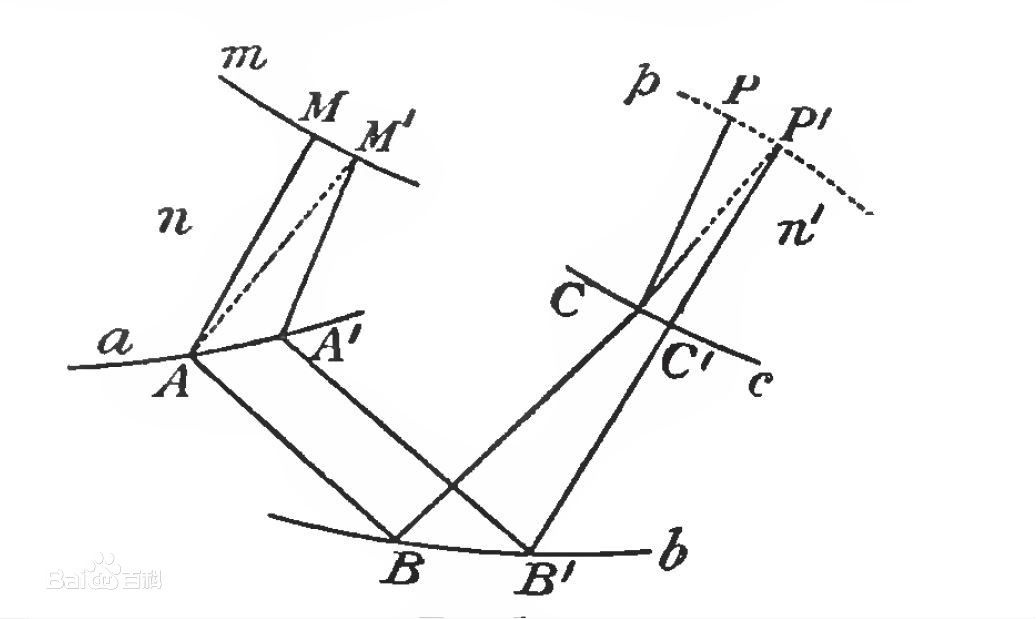
\includegraphics[clip,scale=0.18]{assets/fig7.jpg}
\end{minipage}
\caption{马吕斯定律原理示意图}
\label{figure.6}
\end{figure}

\textbf{(2) 公式推导}

两个偏振器的透射方向之间的角度为$\alpha$。通过偏振器的偏振光振幅为$A_{0}$，通过偏振器的振幅为A。那么我们有：
\begin{eqnarray}
    A=A_{0} \cos \alpha 
\end{eqnarray}

因为检测器检测的是光强，光强I为：
\begin{eqnarray}
I=A^{2} 
\end{eqnarray}

继续推导得：
\begin{eqnarray}
    I=\left (A_{0}\cos {\alpha }   \right ) ^{2} =I_{0} \cos ^{2} \alpha 
\end{eqnarray}

\vspace{0.5cm}
\textbf{四、实验内容与步骤}

\textbf{确定光源的偏振性并验证马吕斯定律}

A. 将激光器和光强检测器放在导轨上，然后打开光强检测器电源开关，当导轨上没有其他组件时，使激光垂直进入光强检测器。

B. 放置偏转器，调整偏转器的高度使激光通过其中心；调整偏转器的角度使光强读数最大，从最大光强位置旋转$90^\circ$，逐一改变偏转器的角度，每$10^\circ$记录一组数据，并根据获得的数据确定光源的偏振状态。
\begin{figure}[h]
    \centering
    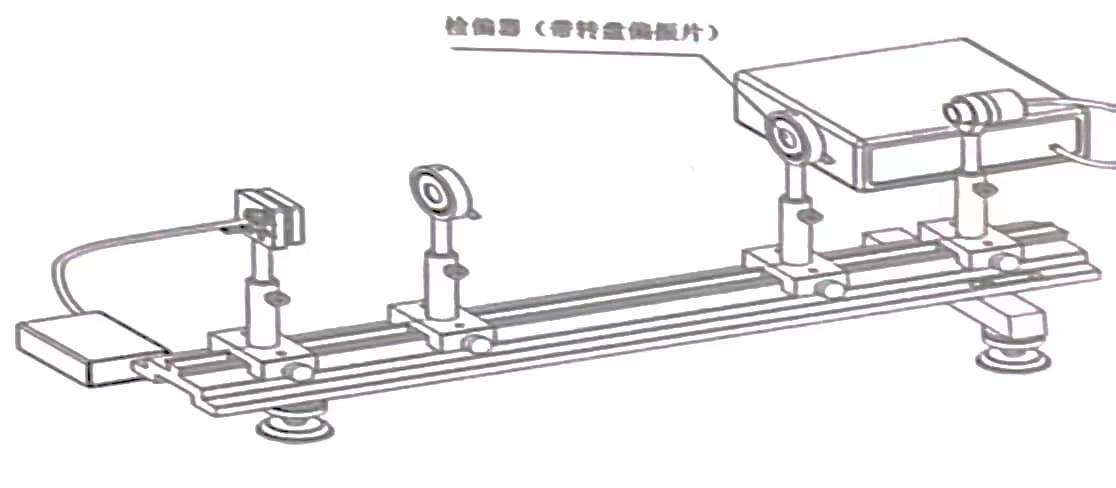
\includegraphics[clip,scale=0.2,trim={0 0 0 0}]{assets/fig9.jpg}
    \caption{操作演示图}
    \label{figure.8}
\end{figure}

C. 如果得出光源是线偏振光，使用这些数据绘制$I\sim \left ( \cos \theta  \right ) ^{2}$图表以验证马吕斯定律。

D. 如果光源不是线偏振的，将偏振器设回光强读数最大的位置，放入检测器并调整检测器使光强读数最大，从这个位置开始旋转$90^\circ$，每次改变检测器的角度并每$10^\circ$记录一组数据。最后，利用获得的数据验证马吕斯定律。

\vspace{0.5cm}
\textbf{五、数据处理}

\textbf{马吕斯定律的验证}

根据实验步骤，测量偏振光通过偏振器后强度随角度的变化。记录数据如下：
\begin{center}
    \begin{tabular}{ccc}
        \toprule
        序号 & 偏振片2旋转角度(夹角$\theta$) & 光电流值(与光强成正比)($\times 10^{-7}A$)\\
        \midrule
        1 & 初始位置消光时($\theta = 90^\circ$) & 0.01 \\
        2 & 旋转$10^\circ$($\theta = 80^\circ$) & 0.25 \\
        3 & 旋转$20^\circ$($\theta = 70^\circ$) & 0.81 \\
        4 & 旋转$30^\circ$($\theta = 60^\circ$) & 1.92 \\
        5 & 旋转$40^\circ$($\theta = 50^\circ$) & 3.02 \\
        6 & 旋转$50^\circ$($\theta = 40^\circ$) & 4.21 \\
        7 & 旋转$60^\circ$($\theta = 30^\circ$) & 4.87 \\
        8 & 旋转$70^\circ$($\theta = 20^\circ$) & 5.81 \\
        9 & 旋转$80^\circ$($\theta = 10^\circ$) & 6.92 \\
        10 & 旋转$90^\circ$($\theta = 0^\circ$) & 7.18 \\
        \bottomrule
    \end{tabular}
\end{center}

按照马吕斯定律，光强I与$\cos^2\theta$成正比。让我们计算每个角度对应的$\cos^2\theta$值，并与实测光强数据进行比较：

\begin{center}
    \begin{tabular}{cccc}
        \toprule
        夹角$\theta$ & 光强I($\times 10^{-7}A$) & $\cos^2\theta$ & $I/I_{max}$ \\
        \midrule
        $90^\circ$ & 0.01 & 0.000 & 0.001 \\
        $80^\circ$ & 0.25 & 0.030 & 0.035 \\
        $70^\circ$ & 0.81 & 0.117 & 0.113 \\
        $60^\circ$ & 1.92 & 0.250 & 0.267 \\
        $50^\circ$ & 3.02 & 0.413 & 0.421 \\
        $40^\circ$ & 4.21 & 0.587 & 0.586 \\
        $30^\circ$ & 4.87 & 0.750 & 0.678 \\
        $20^\circ$ & 5.81 & 0.883 & 0.809 \\
        $10^\circ$ & 6.92 & 0.970 & 0.964 \\
        $0^\circ$ & 7.18 & 1.000 & 1.000 \\
        \bottomrule
    \end{tabular}
\end{center}

对比理论值$\cos^2\theta$和实验数值$I/I_{max}$，我们可以看到它们大致上是成正比的，尤其是在小角度范围内（如0°到50°）。偏差主要存在于较大角度处，这可能是由于实验误差和仪器精度限制造成的。

为了直观显示关系，我们绘制了$I$与$\cos^2\theta$的关系图：
\begin{figure}[H]
    \centering
    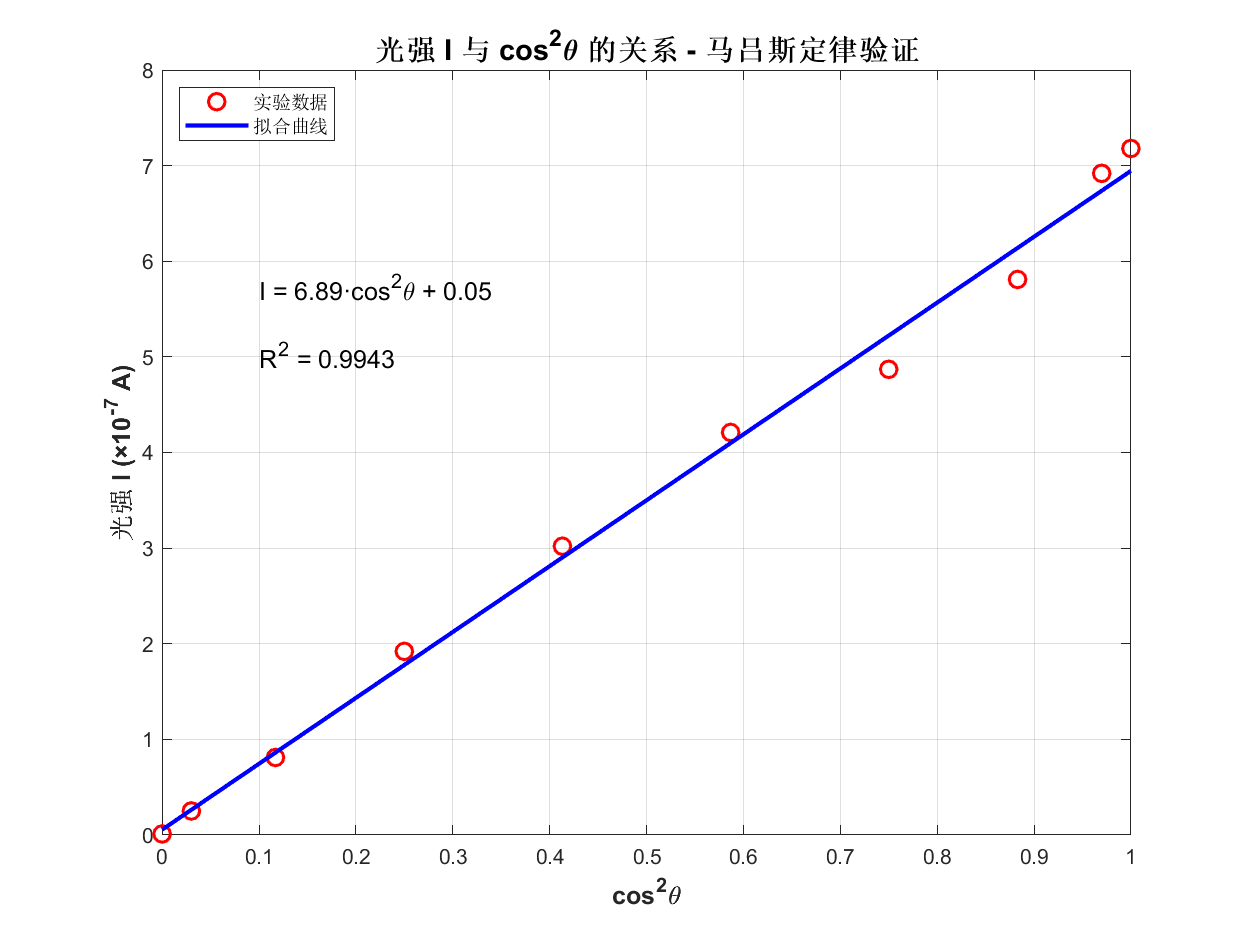
\includegraphics[clip,scale=0.5]{assets/malus_law_fitting.png}
    \caption{$I\sim\cos^2\theta$关系图}
    \label{fig.malus}
\end{figure}

通过最小二乘法拟合，我们可以得到：
\begin{eqnarray}
    I = I_0\cos^2\theta + b
\end{eqnarray}
其中$I_0 \approx 6.89 \times 10^{-7}A$，$b \approx 0.05 \times 10^{-7}A$。

相关系数$R^2 = 0.9943$表明实验数据与马吕斯定律有很好的符合性，验证了马吕斯定律在本实验条件下是成立的。

\textbf{六、结论和分析}

\textbf{1. 实验结论}

马吕斯定律验证：通过测量不同角度下的光强，我们验证了马吕斯定律$I = I_0\cos^2\theta$。实验数据与理论预测具有良好的符合性，相关系数$R^2 = 0.9943$。

\textbf{2. 实验误差分析}

A. 光电流计误差：实验中，光电流计读数不稳定，导致读数困难。

B. 设备误差：激光源无法长时间保持稳定的光源强度，且偏转器和检偏器无法形成完全平行的关系，导致测量中存在一定误差。

C. 环境光误差：尽管实验过程中已经尽量保持环境黑暗，但自然光的存在依然会导致仪器指示与实际激光产生的光强之间存在偏差。

D. 角度测量误差：手动调整偏振器角度可能导致角度读数不够精确。

\textbf{七. 实验感想与改进}

A. 使用更稳定的光源和更精确的测量设备，减少系统误差。

B. 在暗室中进行实验，减少环境光干扰。

C. 增加测量角度点的密度，特别是在理论与实验值差异较大的角度区域，以更好地研究偏差原因。

D. 使用计算机控制的精密旋转台来调整偏振器角度，减少角度测量误差。

E. 使用高精度光强测量仪器，提高光强测量的准确性。

F. 对于数据处理，采用更复杂的拟合模型，考虑非理想因素的影响，如杂散光和仪器背景值。

\end{document}
